\documentclass{article}

\usepackage{algorithm, algpseudocode}
\usepackage{graphicx}

\algnewcommand{\algorithmicforeach}{\textbf{for each}}
\algdef{SE}[FOR]{ForEach}{EndForEach}[1]
{\algorithmicforeach\ #1\ \algorithmicdo}% \ForEach{#1}
{\algorithmicend\ \algorithmicforeach}% \EndForEach
\usepackage{minted} 

\title{Quantitative Sampling for \\ \texttt{Probabilistic Assert Failures}}
\author{Sumit Lahiri \\ \texttt{IIT Kanpur}}

\begin{document}
\maketitle

We try to formulate a way to compute path probabilities using \texttt{symbolic execution} and \texttt{testing} based technique. 

\begin{minted}{c} 
int main(void)
{
	int a; // unintialized
	int d = std::uniform_distribution<rd_seed>(0, 650);
	
	// forall variable : (INT_MIN to INT_MAX)
	klee_make_symbolic(&a, sizeof(a), "a_sym");
	
	// PSE variable : Uniformly distributed [0 to 650]
	make_pse_symbolic<int>(&d, sizeof(d), "d_prob_sym", 0, 650);
	
	int c = a + 100;
	
	// case 1 : Pure Forall Predicate
	if (a > 50) {
	  c = a + 75;
	} else {
	  c = a - 75;
	}
	
	// case 2 : Pure PSE Predicate
	if (d > 60) d = 250;
	
	// case 3 : Dependence Case
	if (c > d) c = d;

	// Probabilistic query : assert(P(c != d) < 0.5)
	// Optimize here : 
	//	Optimal value of forall variable 'a' 
	//        such that P(c != d) is close to 0.5 	
	return 0;
}
\end{minted}

\begin{algorithm}[H]
	\caption{Candidates : (Testing Based Estimation)}
	\begin{algorithmic}[1]
		\ForEach{$p \in Paths$}%
		\State $c := ConstraintSet(p)$ \algorithmiccomment{Path Constraints for p}
		\State $m := Optimize(query,  c)$ \algorithmiccomment{solution for the path constraints}
		\State $concreteSet = \{ \}$
		\ForEach{$v \in ForallVars(p)$} \algorithmiccomment{ForallVars p $\rightarrow $ forall} %
		\State $concreteSet.append(\{key : v, val : m[v]\})$ \algorithmiccomment{Candidate Values}
		\EndForEach
		\State $executeCV(program, concreteSet)$
		\EndForEach
	\end{algorithmic}
\end{algorithm}

\begin{algorithm}[H]
	\caption{executeCV : PSE Sampled Normal Execution}
	\begin{algorithmic}[1]
		\Function{executeCV}{$P : program, C : concreteSet$}
		\ForEach{$v \in ForallVars(p)$}%
		\State value(v) := concreteSet(v) \algorithmiccomment{Use values from ConcreteSet}
		\EndForEach
		\State ... \algorithmiccomment{proceed with normal execution}
		\EndFunction
	\end{algorithmic}
\end{algorithm}

For the sample program given above, we first resort to using \texttt{symbolic execution} to generate \texttt{path constraints} for all the feasible paths that this program can take and then convert the \texttt{path constraints} into an \texttt{formal logic} optimization problem that gives an \texttt{assignment} to \texttt{forall} variables such that it leads to optimum violation of the $query$.

\begin{minted}{python}
def generateCandidates(k: int): # Candidates Algorithm
	opt = z3.Optimize()
	a = z3.Int("a_sym")
	d = z3.Int("d_prob_sym")
	
	opt.add(d >= 0)
	opt.add(d <= 650)
	opt.add(a > 50)
	opt.add(z3.Not(d > 60))
	opt.add(a + 75 > d)

	opt.maximize(a - d - 75) 	# Query to optimize
	n = 0
	while opt.check() == z3.sat and n != k:
		m = opt.model()
		n += 1
		print("%s = %s" % (a, m[a]))
		print("%s = %s" % (d, m[d]))
		opt.add(a != m[a])
\end{minted}

We now explore a slightly different example which is more involved in terms of the constraints and query that the user can pose at the end of the \texttt{symbolic execution}. In the below example we bound the values for \texttt{foralls} for example sake. 

\begin{minted}{c}
// forall variable
klee_make_symbolic(&a, sizeof(a), "a_sym");       // [0, 1]
klee_make_symbolic(&c, sizeof(b), "c_sym");       // [1, 10]
klee_make_symbolic(&d, sizeof(c), "d_sym");       // [0, 5]
klee_make_symbolic(&win, sizeof(win), "win_sym"); // win == 1

// PSE variable
make_pse_symbolic<int>(&b, sizeof(b), "b_prob_sym", 0, 1);
make_pse_symbolic<int>(&e, sizeof(e), "e_prob_sym", 1, 6);

klee_assume(a >= 0 && a <= 1);
klee_assume(c >= 1 && c <= 10);
klee_assume(d >= 0 && d <= 5);

if (a > b)				     // maximize a
{
	if (c + e < 15)			// minimize c
	{
		win = 1;			
		win_ones++;
	}
	else
	{
		win = 0;
		win_zeros++;
	}
}
else
{
	if (d + e > 1)			// maximize d
	{
		win = 1;
		win_ones++;
	}
	else
	{
		win = 0;
		win_zeros++;
	}
}
\end{minted}

Below we show a sample of the type of the \texttt{queries} that a user can make in the context of the example shown above. 

\begin{minted}{c}
	assert(P(win == 1) > 0.8);
\end{minted}

Based on the query posed, we get \texttt{candidate} models by converting the code into a \texttt{optimization} query and solve this optimization problem using any off-the-shelf 
\texttt{SMT Solver} to get model values for the forall variables that contribute to maximum 
violation of the \texttt{query} constraint. 

Based on the example we do the following \texttt{optimizations}. one on \texttt{Path 1} and the other on \texttt{Path 3} where \texttt{win == 1} 

\begin{minted}{c}
	Path 1 : maximize((a - b) + 11 - (c + e))
\end{minted}

\begin{minted}{c}
	Path 3 : maximize((b - a) + (d + e) - 1)
\end{minted}

On the other two paths, we \texttt{minimize} the same. \texttt{win == 1} on the \texttt{green} edged paths. \\

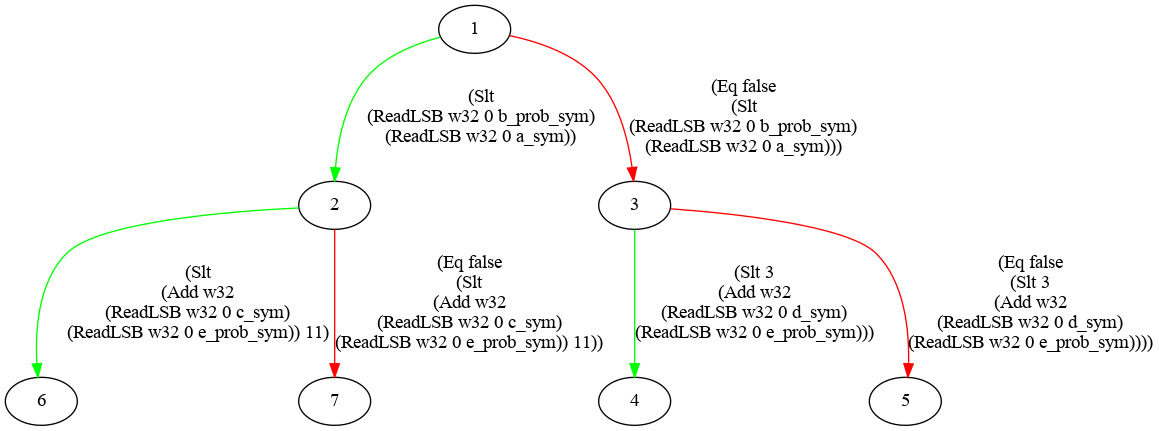
\includegraphics[scale=0.35]{exectree1.png} 

\begin{minted}{c}
Path 1 : [And(a_sym >= 0, a_sym <= 1), And(c_sym >= 1, c_sym <= 10),
 And(d_sym >= 0, d_sym <= 5), And(b_prob_sym >= 0, b_prob_sym <= 1), 
 And(e_prob_sym >= 1, e_prob_sym <= 6), win_sym == 1, b_prob_sym < 
 a_sym, c_sym + e_prob_sym < 15]
	Model : 1
		a_sym = 1
		c_sym = 1
		d_sym = 0
	Model : 2
		a_sym = 1
		c_sym = 2
		d_sym = 0
	Model : 3
		a_sym = 1
		c_sym = 3
		d_sym = 0
Path 2 : [And(a_sym >= 0, a_sym <= 1), And(c_sym >= 1, c_sym <= 10), 
And(d_sym >= 0, d_sym <= 5), And(b_prob_sym >= 0, b_prob_sym <= 1), 
And(e_prob_sym >= 1, e_prob_sym <= 6), b_prob_sym < a_sym, Not(c_sym 
+ e_prob_sym < 15)]
	Model : 1
		a_sym = 1
		c_sym = 9
		d_sym = 0
	Model : 2
		a_sym = 1
		c_sym = 10
		d_sym = 0
Path 3 : [And(a_sym >= 0, a_sym <= 1), And(c_sym >= 1, c_sym <= 10), 
And(d_sym >= 0, d_sym <= 5), And(b_prob_sym >= 0, b_prob_sym <= 1), 
And(e_prob_sym >= 1, e_prob_sym <= 6), win_sym == 1, Not(b_prob_sym 
< a_sym), d_sym + e_prob_sym > 1]
	Model : 1
		a_sym = 0
		c_sym = 1
		d_sym = 0
	Model : 2
		a_sym = 0
		c_sym = 2
		d_sym = 0
	Model : 3
		a_sym = 0
		c_sym = 3
		d_sym = 1

		...
\end{minted}

Here \texttt{P(win == 1)} is the query of interest to us so we optimize along those paths where this condition holds. \\   

We now do a \texttt{transformation} pass over the program and instrument the count of the given \texttt{condition} failing. In the \texttt{transforamtion} pass, we make the \texttt{program} take values that we find as \texttt{candidate} models upon following \texttt{Algorithm 1}

\begin{minted}{c}
// Take in candidate vector for [foralls]
scanf("%d", &a); // [0, 1]
scanf("%d", &c); // [1, 10]
scanf("%d", &d); // [0, 5]

// // PSE variable : Random Sampling
std::default_random_engine generator;
std::uniform_int_distribution<int> distribution1(0, 1); // b
std::uniform_int_distribution<int> distribution2(1, 6); // e

while (term_count--) // term_count > 500000 (large sample)
{
	b = distribution1(generator);
	e = distribution2(generator);
	
	if (a > b) { // 
		if (c + e < 15) {
			win = 1;
			win_ones++;
		} else {
			...
		}
	} else {
		if (d + e > 1) {
			win = 1;
			win_ones++;
		} else {
			...
		}
	}
	run++;
} 

// The probabilistic assert is the following
// assert(P(win == 1) >= 0.8), where P(win == 1) win_ones/run;

\end{minted}

We tweaked the values in such a way that for a very small number of candidate vectors the \texttt(probabilistic) assert fails and our algorithm must now catch that. Indeed we find that for the following assignments to \texttt{forall} variables, the assert fails.

\begin{minted}{c}
	Fail : P(win == 1)  :  0.754100
		Vals -> a : 1, c : 10, d : 0
\end{minted}

For other \texttt{candidate} vectors, we find that the \texttt{probabilistic} asserts actually hold and will not cause a violation during execution under normal condiditons. We show the results of some of the winning cases here. 

\begin{minted}{c}
	Pass : P(win == 1)  :  1.000000
		Vals -> a : 0, c : 7, d : 4
	Pass : P(win == 1)  :  1.000000
		Vals -> a : 1, c : 4, d : 4
	Pass : P(win == 1)  :  1.000000
		Vals -> a : 1, c : 1, d : 3
	Pass : P(win == 1)  :  1.000000
		Vals -> a : 0, c : 6, d : 4
	Pass : P(win == 1)  :  0.834900
		Vals -> a : 0, c : 7, d : 0
	Pass : P(win == 1)  :  0.834900
		Vals -> a : 0, c : 2, d : 0
	Pass : P(win == 1)  :  1.000000
		Vals -> a : 0, c : 10, d : 2
	Pass : P(win == 1)  :  0.917800
		Vals -> a : 1, c : 3, d : 0
			...
\end{minted}
\end{document}